\documentclass[11pt, french]{article}
\usepackage{calc}
\usepackage{eso-pic}

\newlength{\PageFrameTopMargin}
\newlength{\PageFrameBottomMargin}
\newlength{\PageFrameLeftMargin}
\newlength{\PageFrameRightMargin}

\setlength{\PageFrameTopMargin}{1.5cm}
\setlength{\PageFrameBottomMargin}{1cm}
\setlength{\PageFrameLeftMargin}{1cm}
\setlength{\PageFrameRightMargin}{1cm}

\makeatletter

\newlength{\Page@FrameHeight}
\newlength{\Page@FrameWidth}

\AddToShipoutPicture{
  \thinlines
  \setlength{\Page@FrameHeight}{\paperheight-\PageFrameTopMargin-\PageFrameBottomMargin}
  \setlength{\Page@FrameWidth}{\paperwidth-\PageFrameLeftMargin-\PageFrameRightMargin}
  \put(\strip@pt\PageFrameLeftMargin,\strip@pt\PageFrameTopMargin){
    \framebox(\strip@pt\Page@FrameWidth, \strip@pt\Page@FrameHeight){}}}

\makeatother
%%%%%%%%%%%%%%%%%%%%%%%%%%%%%%%%%%%%%%%%%%%%%%%%%%%%%
% Importation des paquets
%%%%%%%%%%%%%%%%%%%%%%%%%%%%%%%%%%%%%%%%%%%%%%%%%%%%%
\usepackage[utf8]{inputenc}
\usepackage{helvet}
\usepackage{natbib}
\usepackage{graphicx}
\usepackage{libertine}
\usepackage{eso-pic}
\usepackage{hyperref} % allow to write hyperlink (open the url)
\usepackage{titlesec} % allow to change fontsize of the different section
\usepackage{tabularx} % allow to create tables with fixed length
\usepackage{listings} % code highlighting
\usepackage{xcolor}
\usepackage{amsmath}
\usepackage{amssymb}

\usepackage[a4paper,margin=1in]{geometry}
\definecolor{LightGray}{gray}{0.9}


%%%%%%%%%%%%%%%%%%%%%%%%%%%%%%%%%%%%%%%%%%%%%%%%%%%%%
% Definition des commandes
%%%%%%%%%%%%%%%%%%%%%%%%%%%%%%%%%%%%%%%%%%%%%%%%%%%%%
% Permet de définir une image en arrière plan
\newcommand\BackgroundPic{%
\put(0,0){%
\parbox[b][\paperheight]{\paperwidth}{%
\vfill
\centering
\includegraphics[width=\paperwidth,height=\paperheight]{background-42-ai.png}%
\vfill
}}}

% Définition de la commande pour faire un snippet de code inline
\newcommand{\inlsnippet}[1]{\colorbox{gray!10}{\mbox{\textcolor{pink}{#1}}}}

% Modification of the style of hyperlink, to be visible
\hypersetup{
    colorlinks=true,
    linkcolor=blue,
    filecolor=magenta,      
    urlcolor=cyan,
}

%%%%%%%%%%%%%%%%%%%%%%%%%%%%%%%%%%%%%%%%%%%%%%%%%%%%%%%%%%%%%%%%%%%%%%%%%%%
% Definition of black backgrounded Python code snippet
%%%%%%%%%%%%%%%%%%%%%%%%%%%%%%%%%%%%%%%%%%%%%%%%%%%%%%%%%%%%%%%%%%%%%%%%%%%
\definecolor{pink}{HTML}{ff33cc}
\definecolor{codewhite}{HTML}{ffffff}
\definecolor{codegreen}{HTML}{00e600}
\definecolor{codelemon}{HTML}{99ff99}
\definecolor{codegray}{HTML}{bfbfbf}
\definecolor{codepurple}{HTML}{9933ff}
\definecolor{codeblue}{HTML}{0099ff}
\definecolor{codered}{HTML}{ff3333}
\definecolor{bg}{HTML}{000000}

\lstdefinestyle{nightly}{
    language=Python,
    backgroundcolor=\color{bg},   
    commentstyle=\fontfamily{cmss}\color{codegreen},
    keywordstyle=\fontfamily{cmss}\color{codeblue},
    otherkeywordstyle=\fontfamily{cmss}\color{codered},            
    numberstyle=\fontfamily{cmss}\small\color{codegray},
    stringstyle=\fontfamily{cmss}\color{codepurple},
    basicstyle=\fontfamily{cmss}\small\color{codewhite},
    emph={def,is,not,in,False,True,as,and,or,from},
    emphstyle={\fontfamily{cmss}\small\color{pink}},
    emph={[2]MyClass,__init__,__repr__,__print__},
    emphstyle={[2]\fontfamily{cmss}\small\color{codered}},
    emph={[3]str,float,tuple,int,list},
    emphstyle={[3]\fontfamily{cmss}\small\color{codelemon}},
    breakatwhitespace=false,         
    breaklines=true,                 
    captionpos=b,                    
    keepspaces=true,                 
    numbers=left,                    
    numbersep=5pt,                  
    showspaces=false,                
    showstringspaces=false,
    showtabs=false,                  
    tabsize=2
}
%%%%%%%%%%%%%%%%%%%%%%%%%%%%%%%  End of definition  %%%%%%%%%%%%%%%%%%%%


%%%%%%%%%%%%%%%%%%%%%%%%%%%%%%%%%%%%%%%%%%%%%%%%%%%%%
% Titre, date, auteur
%%%%%%%%%%%%%%%%%%%%%%%%%%%%%%%%%%%%%%%%%%%%%%%%%%%%%

\author{} %\author{42-AI}
\title{Practise sheet}
%\maketitle

%%%%%%%%%%%%%%%%%%%%%%%%%%%%%%%%%%%%%%%%%%%%%%%%%%%%%
% Début du document
%%%%%%%%%%%%%%%%%%%%%%%%%%%%%%%%%%%%%%%%%%%%%%%%%%%%%
\begin{document}


%%% >>>>> Page de garde
\vspace*{2cm}
\begin{center}
    \textsc{\fontsize{40}{48} \bfseries Practise Sheet 2}\\[0.6cm]
    \textsc{\fontsize{40}{48} \bfseries Analysis}\\[0.3cm]
\end{center}
\vspace{3cm}

\begin{figure}[!h]
\center

\includegraphics[scale=0.5]{logo-42-ai.png}
\label{fig:1st_page_logo_42ai}
\end{figure}

\vspace*{2cm}
\begin{center}
    \textsc{\fontsize{32}{48} \bfseries Les fonctions de référence}\\[0.6cm]
\end{center}
\vspace{3cm}

\pagenumbering{gobble}
\newpage


%%% >>>>> Document body
%\begin{center}
%\chapter{\fontsize{30}{36} \selectfont Practise Sheet 1 - Les bases des fonctions}
%\end{center}
%\vspace{10mm}



\section*{Objectifs:}
L'objectif principal de cette série d'exercices est de vous familiariser avec un ensemble de fonctions classiques.

\section*{Exercice 1: Échauffement}
Le but de l'exercice est d'améliorer l'acquisition des connaissances sur les fonctions.
### Partie 1: Images et antécédents
Rien de nouveau ici, juste des fonctions différentes.

\begin{enumerate}

    \item Donner les ensembles de définition et image des fonctions suivantes:
    \begin{equation*}
        f(x) = x^2, \quad g(x) = \frac{1}{x} \\
        h(x) = x + 1, \quad i(x)=\sqrt{x}
    \end{equation*}
    Pourquoi la fonction $g$ n'est pas définie en $x=0$ ?
    \item Calculer les images par les fonctions précédentes, des nombres présents dans la liste (si c'est possible) $X = [-5, -4, -3, -2, -1, 0, 1, 2, 3, 4, 5]$
    \item Tracer les représentations graphiques des fonctions $f$, $g$, $h$ et $i$.
    \item Considérons la fonction $f_1$:
    \begin{equation*}
        f_1(x) = \sqrt{x}+2
    \end{equation*}
    \begin{enumerate}
       \item Déterminer les antécédents des valeurs suivantes: 2, 4, 14 et 14.5.
       \item Existe-t-il des antécédents pour les valeurs appartenant à l'intervalle $]\infty ; 0]$ ? Pourquoi ?
    \end{enumerate}
    \item Même chose pour la fonction $f_2$:
    \begin{equation*}
        f_2(x) = \sqrt{x+4} 
    \end{equation*}
    \begin{enumerate}
       \item Déterminer les antécédents des valeurs suivantes: 0, 2, 4, 14 et 25.
       \item Existe-t-il des antécédents pour les valeurs appartenant à l'intervalle $[-4 ; 0]$ ?
       \item Sur quel intervalle la fonction $f_2$ n'est pas définie ?
    \end{enumerate}
    \item De même que pour la fonction $f_3$:
    \begin{equation*}
        f_3 = \frac{1}{4}x^2
    \end{equation*}
    \begin{enumerate}
       \item Déterminer les antécédents des valeurs 2, 3, 4, 5 et 6.
       \item Donner le domaine image de la fonction $f_3$.
    \end{enumerate}
    \item Et enfin pour la fonction $f_4$:
    \begin{equation*}
        f_4 = 2x^2 - 16
    \end{equation*}
    \begin{enumerate}
       \item Déterminer les antécédents des valeurs 2, -16, -8, 0 et 34.
       \item Donner le domaine image de la fonction $f_4$.
    \end{enumerate}
\end{enumerate}
\vspace{2cm}

\section*{Exercice 2: Tableau de valeurs et représentation graphique}
Nous continuons l'étude des fonctions avec encore des tableaux de valeurs et les représentations graphiques.\\
Nous allons également aborder la notion de parité pour les fonctions.\\
L'objectif est de renforcer votre capacité d'analyse sur les fonctions, développer votre intuition en quelque sorte.

\noindent\rule{\textwidth}{1pt}
Concernant la parité.
Les fonctions qui sont possiblement paires impaires doivent au préalable avoir un \textbf{domaine de définition $D_f$} que l'on qualifie de \textbf{symétrique}.\
Un domaine de définition (\textit{plus largement un ensemble}) est symétrique si pour \textbf{tout nombre de ce domaine, son opposé appartient aussi au domaine}.\
Toute fonction dont le domaine de définition n'est pas symétrique ne peut ni être paire ni impaire.\

Enfin,\
\paragraph{une fonction $f$ est dite paire} si son domaine de définition $D_f$ est symétrique et si pour tout $x\in D_f$:
\begin{equation*}
    f(-x) = f(x)
\end{equation*}
\paragraph{une fonction $f$ est dite impaire} si son domaine de définition $D_f$ est symétrique et si pour tout $x\in D_f$:
\begin{equation*}
f(-x) = - f(x)
\end{equation*}

Pour finir sur la parité, il peut être noté une particularité graphique.
Les fonctions \textbf{paires} sont \textbf{symétriques par rapport à l'axe des ordonnées}.\
Quant aux fonctions \textbf{impaires}, elles sont \textbf{symétriques par rapport au point d'origine du repère} (point de coordonnées $(0; 0)$).

\begin{figure}[!h]
\center
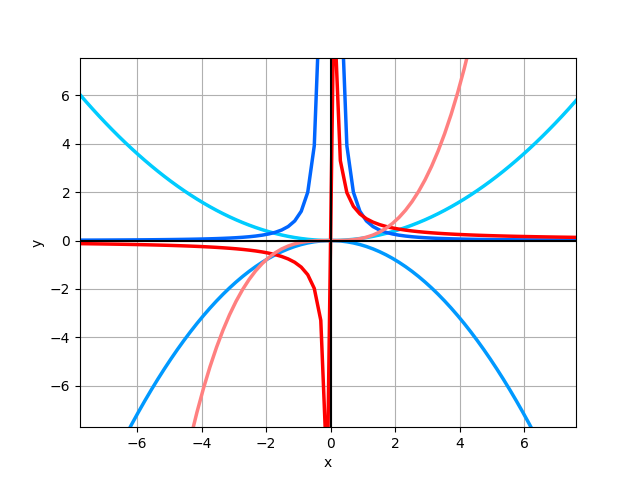
\includegraphics[scale=0.6]{assets/serie_2_exo_2_figure_1.png}
\caption{Les courbes en bleues sont des représentations graphiques de fonctions paires et les courbes en rouges/oranges sont les représentations graphiques de fonctions impaires.}
\label{fig:p_s_2_exo1-fig1}
\end{figure}

\subsubsection*{Remarques:}
Vous vous demandez probablement à quoi cela peut vous servir pour faire du ML. Et bien cela peut vous aider à choisir un ou plusieurs modèles avant de les entraîner.\\
Notamment, après une étape de standardisation des données, il est possible d'observer si les données peuvent être modélisé par une fonction paire, impaire ou n'ayant sans parité.\\
Un choix cohérent de modèle participe à l'obtention d'un score plus faible une fois le modèle entraîné.
\noindent\rule{\textwidth}{1pt}


\subsection*{Partie 1:}
Vous allez vous exercer à la reconnaissance de la parité des fonctions visuellement et à partir de l'expression algébrique.

\begin{enumerate}
    \item Pour chacune les fonctions représentées ci dessous, préciser lesquelles sont paires, impaires où ni l'une ou l'autre.
    \begin{figure}[!h]
        \center
        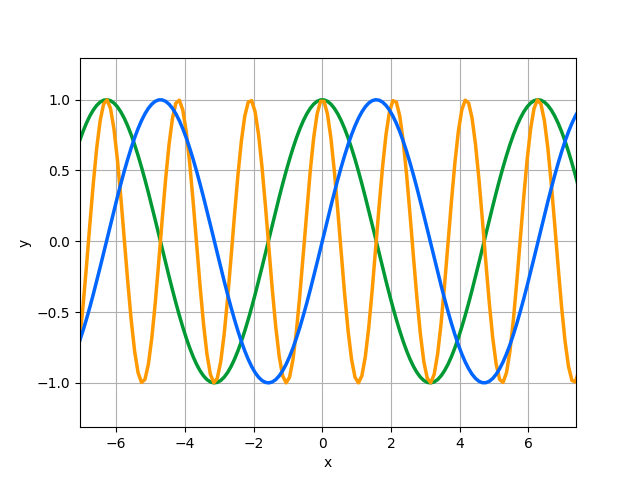
\includegraphics[scale=0.32]{assets/serie_2_exo_2_figure_2.png}
        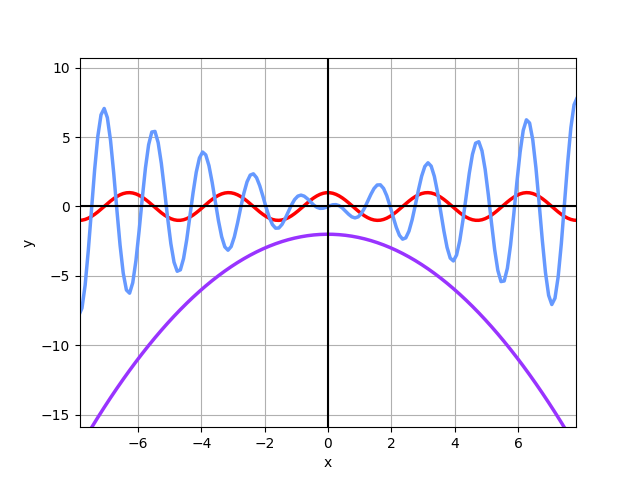
\includegraphics[scale=0.32]{assets/serie_2_exo_2_figure_3.png}
        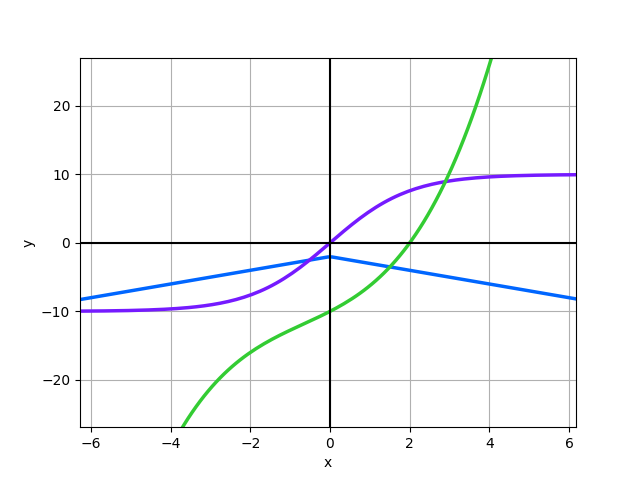
\includegraphics[scale=0.32]{assets/serie_2_exo_2_figure_4.png}
        \label{fig:p_s_2_exo2-fig123}
    \end{figure}
    \item À partir des expressions algébriques des fonctions suivantes, déterminer lesquelles sont paires, impaires ou ni l'un ni l'autre. Le domaine de définition des différentes fonctions est $\mathbb{R}$.
    \begin{align*}
    \begin{matrix}
    f_1(x) = x^2 +4, & f_2(x) = -2x - 3 & f_3(x) =  x^2 + 1\\
    f_4(x) = -2x^2 + x & f_5(x) = \frac{-2}{x} & f_6(x) = \frac{1}{x^2} \\
    f_7(x) = \frac{2}{x + 1} & f_8(x) = \sqrt{|x|} & f_9(x) = 3x^3\sqrt{|x|}
    \end{matrix}
    \end{align*}
\end{enumerate}

\subsection*{Partie 2: Coding time !}
Coder une fonction python capable de dire si une fonction est possiblement paire ou impaire ou sans parité.

Il vous faut prendre en compte 2 choses:
\begin{itemize}
    \item le domaine de définition de la fonction,
    \item le \textit{"comportement"} de la fonction pour $x$ et $-x$.
\end{itemize}

Dans la librairie \inlsnippet{Sympy}, il n'y a (à la connaissance de l'auteur des exercices) pas de fonction permettant de donner le domaine de définition de la fonction, uniquement le domaine de continuité (\inlsnippet{continuous\_ domain}).
Ainsi, vous ne devrez pas vérifier la condition de symétrie du domaine de définition de la fonction.

\begin{enumerate}
    \item Coder une fonction qui permet de dire (sans que ça soit démontrer, donc ça reste une supposition) si la fonction est paire, impaire ou sans parité.
    \begin{lstlisting}[style=nightly]
    def parity_guess(f, nb_list):
        """
        Arguments:
            f : a function or an expression.
            nb_list : a list of positive numbers.
        Description:
            The function calculate the image by the function of each numbers and its opposite values.
            Then the function compares the 2 lists of images to conclude on   the guess of the parity.
        Return:
            "La fonction semble paire"
            "La fonction semble impaire"
            "La fonction n'a pas de parité"
        """
    \end{lstlisting}
    \item \textbf{**Version dure : (facultatif)}
    Une version améliorer du code peut être faite en prenant en compte le domaine de définition.\\
    Une manière d'obtenir le domaine de définition est de résoudre les 3 équations suivantes:
    \begin{equation*}
    \begin{matrix}
        f(x) & > & 0 \\
        f(x) & = & 0 \\
        f(x) & < & 0 \\
    \end{matrix}
    \end{equation*}
    et d'unir les intervalles de chaque équation.\
    Il faut ensuite vérifier que le domaine est symétrique.
    Ensuite il faut vérifier si l'expression de la fonction est invariable en substituant $x$ par $-x$ ou bien déterminer que les expressions de $f(x) +f(-x)$ ainsi que $f(x) - f(-x)$.
    \textit{(Un peu compliqué, donc je ne le recommande que pour ceux les plus motivés et/ou à l'aise)}\
    Voici un petit coup de pouce pour ceux qui tenterai de le faire, vous pouvez regarder les éléments suivants.
   \begin{lstlisting}[style=nightly]
    sympy.Symbol
    sympy.Lambda
    sympy.Intersection
    sympy.Union
    sympy.expr
    sympy.subs
   \end{lstlisting}
\end{enumerate}
\vspace{2cm}

\section*{Exercice 3 : Trouver le bon modèle}
Pour les 2 parties suivantes, l'objectif est de trouver les modèles les plus pertinents.

\subsection*{Partie 1:}
Une entreprise produit et vend des boules de Noël. Le prix unitaire est fixé entre $1$ et $10$ €. Le gérant a effectué une étude sur la recette (en milliers d'euros) issue de différentes boules en fonction du prix de vente de celles-ci (vous trouverez les données dans le fichier data\_analysis\_practise\_sheet\_2\_ex03.csv)

\begin{figure}[!h]
    \center
    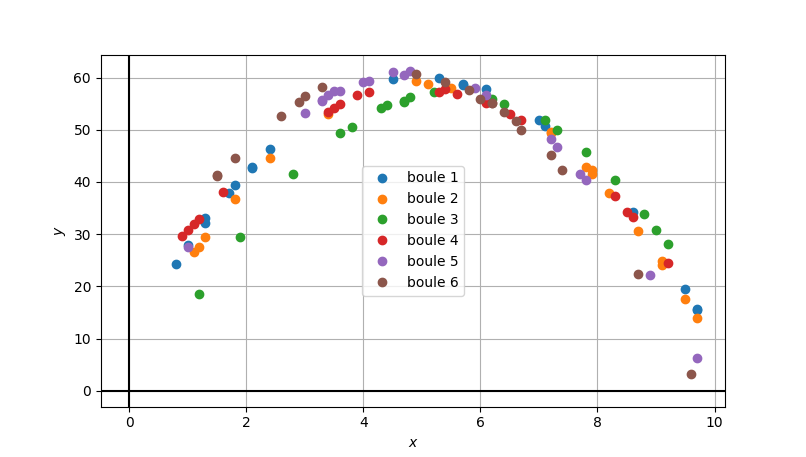
\includegraphics[scale=0.7]{assets/serie_2_exo_3_figure_5.png}
    \label{fig:p_s_2_exo3-fig1}
\end{figure}

\begin{itemize}
    \item Tracer l'évolution de la recette quotidienne en fonction du prix de vente unitaire pour chaque boule de Noël.
    \item Tracer l'évolution de la recette quotidienne moyenne en fonction du prix de vente unitaire pour toutes les boules de Noël.
    \item Proposer un modèle pouvant décrire l'évolution de la recette moyenne.
    \item Représenter le modèle avec les données et plusieurs autres modèles que vous jugez moins bon pour prédire la l'évolution de la recette quotidienne.
\end{itemize}

\subsection*{Partie 2:}
La quantité de boules de Noël vendu dans plusieurs magasins entre le 1$^\text{er}$ novembre et le 10 décembre a été enregistré et les données son représentée dans le graphique suivant.

\begin{figure}[!h]
    \center
    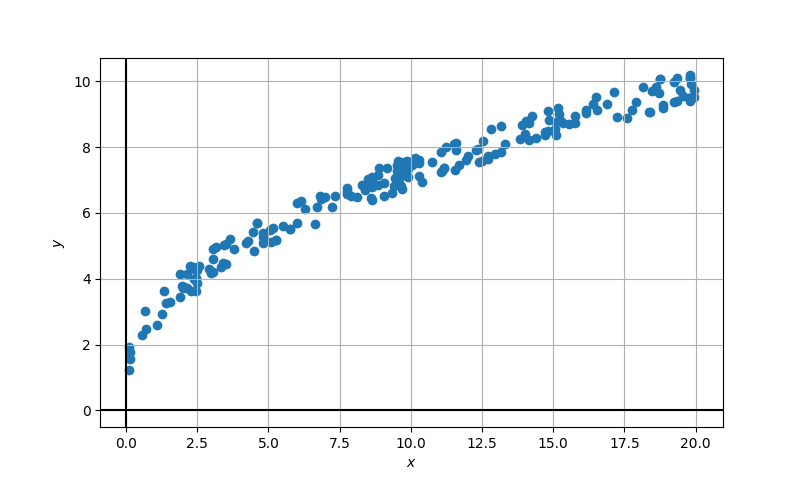
\includegraphics[scale=0.7]{assets/serie_2_exo_3_figure_6.png}
    \label{fig:p_s_2_exo3-fig1}
\end{figure}

\begin{itemize}
    \item Tracer vous même les données.
    \item Proposer plusieurs modèles qui vous semblent possible.
    \item Tracer ces différents modèles en même temps que les données, conclure sur lequel est le meilleur modèle.
\end{itemize}


%\begin{lstlisting}[style=nightly]
%import numpy as np
%def test_function:
 %   """
 %   Description..
 %   """
 %   for i in range(0,5):
 %       list()
 %       int()
 %       return
 %   
 %   # comment
 %   x = 2
 %   test_function()
%\end{lstlisting}

\end{document}
%%%%%%%%%%%%%%%%%%%%%%%%%%%%%%%%%%%%%%%%%%%%%%%%%%%%%